\documentclass[tikz,border=12pt]{standalone}
\usepackage{fontspec}
\setmainfont{Segoe UI}
\usepackage{amsmath,amssymb}
\usepackage{tikz}

\usetikzlibrary{calc,arrows.meta}

\begin{document}
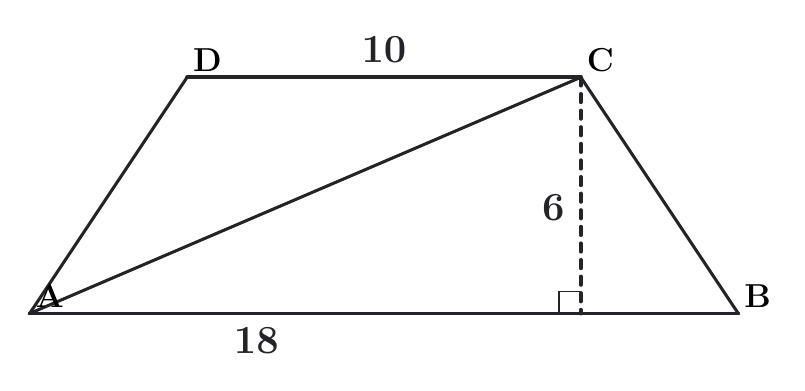
\begin{tikzpicture}[x=1.0000cm,y=1cm,line cap=round,line join=round]
\definecolor{linec0}{RGB}{35,35,40}
\definecolor{linec1}{RGB}{35,35,40}
\definecolor{linec2}{RGB}{35,35,40}
\definecolor{linec3}{RGB}{35,35,40}
\definecolor{linec4}{RGB}{35,35,40}
\definecolor{linec5}{RGB}{35,35,40}
\definecolor{edgecol}{RGB}{35,35,40}
\definecolor{hicol}{RGB}{35,35,40}
\definecolor{angcol}{RGB}{35,35,40}
\coordinate (A) at (0.0000,0.0000);
\coordinate (B) at (9.0000,0.0000);
\coordinate (D) at (2.0000,3.0000);
\coordinate (C) at (7.0000,3.0000);
\coordinate (H) at (7.0000,0.0000);
\draw[line width=1.4pt,color={rgb,255:red,35;green,35;blue,40}] (A) -- (B);
\draw[edgecol,line width=1.1pt] (B) -- (C);
\draw[line width=1.4pt,color={rgb,255:red,35;green,35;blue,40}] (C) -- (D);
\draw[edgecol,line width=1.1pt] (D) -- (A);
\draw[edgecol,line width=1.1pt] (A) -- (C);
\draw[line width=1.4pt,color={rgb,255:red,35;green,35;blue,40},dashed] (C) -- (H);
\draw[edgecol,line width=0.7pt] (7.000,0.280) -- (6.720,0.280) -- (6.720,0.000);
\node[font=\bfseries\Large,text={rgb,255:red,35;green,35;blue,40}] at (2.880,-0.350) {18};
\node[font=\bfseries\Large,text={rgb,255:red,35;green,35;blue,40}] at (4.500,3.350) {10};
\node[font=\bfseries\Large,text={rgb,255:red,35;green,35;blue,40}] at (6.650,1.350) {6};
\node[font=\bfseries\large,inner sep=2pt,anchor=south west] at (0.000,0.000) {A};
\node[font=\bfseries\large,inner sep=2pt,anchor=south west] at (9.000,0.000) {B};
\node[font=\bfseries\large,inner sep=2pt,anchor=south west] at (7.000,3.000) {C};
\node[font=\bfseries\large,inner sep=2pt,anchor=south west] at (2.000,3.000) {D};
\end{tikzpicture}
\end{document}
